\documentclass{beamer}
\usepackage[utf8]{inputenc}
\usepackage{amsfonts, amsmath, amsthm, amssymb, mathtools} 
\usepackage{graphicx} 
\usepackage{xcolor}
\usepackage{float}
\usepackage{hyperref}

\newcommand{\F}{{\mathbb F}}
\newcommand{\Z}{{\mathbb Z}}
\newcommand{\N}{{\mathbb N}}
\newcommand{\R}{{\mathbb R}}

\definecolor{dblue}{rgb}{0.2,0.2,0.7}
\newcommand{\redtext}[1]{{\textcolor{red}{#1}}}
\newcommand{\greentext}[1]{{\textcolor{dgreen}{#1}}}
\newcommand{\bluetext}[1]{{\textcolor{dblue}{#1}}}
\newcommand{\blacktext}[1]{{\textcolor{black}{#1}}}
\newcommand{\remph}[1]{\redtext{\textit{#1}}}
\newcommand{\blemph}[1]{\bluetext{\textit{#1}}}
\newcommand\floor[1]{\lfloor#1\rfloor}
\newcommand\ceil[1]{\lceil#1\rceil}

\def\mathunderline#1#2{\color{#1}\underline{{\color{black}#2}}\color{black}}
\usetheme{Berlin}

\expandafter\def\expandafter\insertshorttitle\expandafter{%
  \insertshorttitle\hfill%
  \insertframenumber\,/\,\inserttotalframenumber}

\title{A Problem from Erd\"os About Products of 2 or 3 Primes}
\subtitle{PUMP Research Symposium}
\author{Trevor Klar \& Eli Moore \\ California State University, Northridge}
\date{April 28th, 2017}

\begin{document}

\begin{frame}
    \titlepage
    \begin{columns}
        \begin{column}{.8\textwidth}
        \end{column}
        
        \begin{column}{.2\textwidth}
            \includegraphics[scale=0.4]{CSUNlogo.png}
        \end{column}
    \end{columns}
\end{frame}
\section{Introduction}
%%%%%%%%%%%%%%%%%%%%%%%%%%%%%%%%%%%%%%%%%%%%%%%%%%
\begin{frame}{Motivation}
    Take two prime numbers, say 2 and 3, and make a list of all the natural numbers which can be formed using only 2 and 3 as factors.
    \[\begin{array}{ ccccccccccccccc }
\Bigg\}\remph{2} & \remph{3} & \remph{4} & \blemph{6} & \remph{8} & \remph{9} & \blemph{12} & ... \\
\remph{\,$2^1$\,} & \remph{\,$3^1$\,} & \remph{\,$2^2$\,} & \blemph{\,$2^13^1$\,} & \remph{\,$2^3$\,} & \remph{\,$3^2$\,} & \blemph{\,$2^23^1$\,} & ...
\end{array}\]
    There is an interesting pattern here: there keep ocurring pairs of numbers which have only 2 or only 3 as a factor. 

\[\begin{array}{ ccccccccccccccc }
... & \blemph{16} & \blemph{18} & \blemph{24} & \remph{27} & \remph{32} & \blemph{36} & ...\\
... & \blemph{\,$2^4$\,} & \blemph{\,$2^13^2$\,} & \blemph{\,$2^33^1$\,} & \remph{\,$3^3$\,} & \remph{\,$2^5$\,} & \blemph{\,$2^23^2$\,} & ...
\end{array}\]
\end{frame}
%%%%%%%%%%%%%%%%%%%%%%%%%%%%%%%%%%%%%%%%%%%%%%%%%%
\begin{frame}{Motivation}
    Does this keep happening?
\[\begin{array}{ ccccccccccccccc }
... & \blemph{1536} & \blemph{1728} & \blemph{1944} & \remph{2048} & \remph{2187} & \blemph{2304} & ...\\
... & \blemph{\,$2^9 3^1$\,} & \blemph{\,$2^6 3^3$\,} & \blemph{\,$2^3 3^5$\,} & \remph{\,$2^{11}$\,} & \remph{\,$3^7$\,} & \blemph{\,$2^8 3^2$\,} & ...
\end{array}\]

    Does it still happen with any primes?
    \[\begin{array}{ ccccccccccccccc }
\remph{59} & \remph{61} & \remph{3481} & \blemph{3599} & \remph{3721} & \remph{205379} & \blemph{212341} & ... \\
\remph{\,$59^1$\,} & \remph{\,$61^1$\,} & \remph{\,$59^2$\,} & \blemph{\,$59^1 61^1$\,} & \remph{\,$61^2$\,} & \remph{\,$59^3$\,} & \blemph{\,$59^2 61^1$\,} & ...
\end{array}\]

\[\begin{array}{ ccccccccccccccc }
%... & \blemph{16} & \blemph{18} & \blemph{24} & \remph{27} & \remph{32} & \blemph{36} & ...\\
... & \blemph{\,$59^3 61^2$\,} & \blemph{\,$59^2 61^3$\,} & \blemph{\,$59^1 61^4$\,} & \remph{\,$61^5$\,} & \remph{\,$59^6$\,} & \blemph{\,$59^5 61^1$\,} & ...
\end{array}\]
\end{frame}
%%%%%%%%%%%%%%%%%%%%%%%%%%%%%%%%%%%%%%%%%%%%%%%%%%
\begin{frame}{Motivation}
     What if you do it with \emph{three} primes (i.e. 2, 3, and 5)?
\[\begin{array}{ ccccccccccccccc }
... & \blemph{18} & \blemph{20} & \blemph{24} & \remph{25} & \remph{27} & \blemph{30} & ... \\
... & \blemph{\,$2^1 3^2$\,} & \blemph{\,$2^2 5^1$\,} & \blemph{\,$2^3 3^1$\,} & \remph{\,$5^2$\,} & \remph{\,$3^3$\,} & \blemph{\,$2^1 3^1 5^1$\,} & ...
\end{array}\]
\end{frame}
%%%%%%%%%%%%%%%%%%%%%%%%%%%%%%%%%%%%%%%%%%%%%%%%%%
\begin{frame}{Question!}
    Paul Erd\"os asked the following question about three distinct primes: If we construct a sequence of all the products of their powers, with the sequence arranged in increasing order, is it true infinitely often that consecutive terms in this sequence are both prime-powers? %Can remove this slide/truncate it/simply state the question out loud, just putting it here so we know to introduce the problem
\end{frame}
%%%%%%%%%%%%%%%%%%%%%%%%%%%%%%%%%%%%%%%%%%%%%%%%%%
\begin{frame}{Definitions}
Let $p,q$ be distinct primes, and let $m,n \in \Z^+$. \\
\begin{block}{Definition}
    \textit{A \remph{pure power} of $p$ is an integer of the form $p^m$.}
\end{block}    
\vspace{.1in} 

\begin{block}{Definition}
    \textit{A \remph{mixed power} of $p$ and $q$ is an integer of the form $p^m q^n$.}
\end{block}   
\vspace{.1in}

\begin{block}{Definition}
    \textit{A \remph{critical pair} of $p$ and $q$ is a pair of pure powers of $p$ and $q$ which do not have a mixed power between them.}
\end{block}    

\end{frame}
%%%%%%%%%%%%%%%%%%%%%%%%%%%%%%%%%%%%%%%%%%%%%%%%%%%%
\section{Early Stages}
\begin{frame}{Developing Intuition}%We could separate this into 3 slides to give examples of each (we can even refer back to the same "example" in the previous slide!)
    
\begin{block}{Lemma 1}
        \textit{If $a_k = q^n$, then $a_{k+1} \neq q^{n+1}$.}
\end{block}
Ex.
\[\begin{array}{ ccccccccccccccc }
... & \blemph{\,$2^4$\,} & \blemph{\,$2^13^2$\,} & \blemph{\,$2^33^1$\,} & \remph{\,$3^3$\,}& ...
\end{array}\]
Here, $3^4$ can't come next, because $3^3<3^32^1<3^4$. 
\end{frame}
%%%%%%%%%%%%%%%%%%%%%%%%%%%%%%%%%%%%%%%%%%%%%%%%%%%%
\begin{frame}{Early Stages}
    \begin{block}{Lemma 2}
        \textit{There exist at most finitely many $a_k = p^m$ such that $a_{k+1} = p^{m+1}$.}
\end{block}
Even in a dramatic example like $p=2$, $q=509$, the sequence starts out all powers of $2$, 
\[\begin{array}{ ccccccccccccccc }
\remph{\,$2^1$\,} & \remph{\,$2^2$\,} & \remph{\,$2^3$\,} & \remph{\,$2^4$\,} & \remph{\,$2^5$\,} &  ...
\end{array}\]
but this can't continue forever. 
\[\begin{array}{ ccccccccccccccc }
\remph{\,$2^7$\,} & \remph{\,$2^8$\,} & \remph{\,$509^1$\,} & \remph{\,$2^9$\,} &  \blemph{\,$2^1 509^1$\,} & ...
\end{array}\]
\end{frame}
%%%%%%%%%%%%%%%%%%%%%%%%%%%%%%%%%%%%%%%%%%%%%%%%%%%%
\begin{frame}{Early Stages}
    \begin{block}{Lemma 3}
        \textit{If $a_k = p^m$ and $a_{k+1} = q^n$, then $m$ and $n$ are relatively prime.}
\end{block}

\textbf{Sketch of Proof.} 
    Suppose for contradiction that gcd$(m,n) = d$. Then $m = m'd$ and $n = n'd$ for some $m', n' \in \N$. Since $p^m = p^{m'd} < q^{n'd} = q^n$, we have $p^{m'} < q^{n'}$. Thus:
    \[
    \begin{array}{rcl}
        p^m & = & p^{m'd}\\
        & = & p^{m'd - m' + m'}\\
        & = & p^{m'(d-1)}p^{m'} \\
        & < & \mathunderline{red}{p^{m'(d-1)}q^{n'}} \\
        & < & q^{n'(d-1)}q^{n'} \\
        & = & q^{n'd} \\
        & = & q^n.
    \end{array}
    \]
\end{frame}
%%%%%%%%%%%%%%%%%%%%%%%%%%%%%%%%%%%%%%%%%%%%%%%%%%%%
\section{Numerical Exploration}
\begin{frame}{The "Tail" of the Sequence of Exponents}
\begin{center}
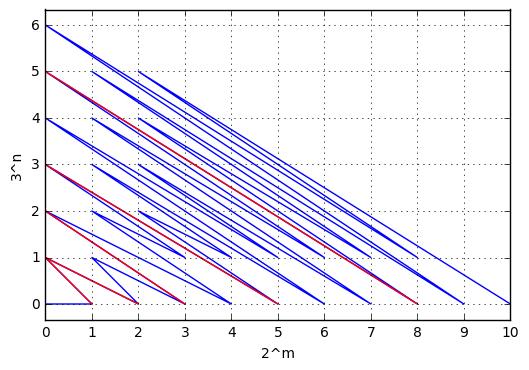
\includegraphics[scale=.48]{slope_plot4.png} 

\scalebox{0.85}{\[\begin{array}{ ccccccccccccccc }
\remph{2} & \remph{3} & \remph{4} & \blemph{6} & \remph{8} & \remph{9} & \blemph{12} & ... \\
\remph{\,$2^1$\,} & \remph{\,$3^1$\,} & \remph{\,$2^2$\,} & \blemph{\,$2^{1}3^1$\,} & \remph{\,$2^3$\,} & \remph{\,$3^2$\,} & \blemph{\,$2^2 3^1$\,} & ...
\end{array}\]}

\end{center}
\end{frame}
%%%%%%%%%%%%%%%%%%%%%%%%%%%%%%%%%%%%%%%%%%%%%%%%%%%%
\begin{frame}{The "Tail" of the Sequence of Exponents}%Another frame
\begin{center}

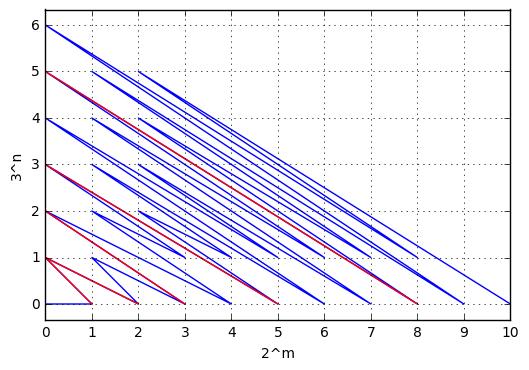
\includegraphics[scale=.48]{slope_plot4.png} 

Notice how the lines seem to approach a constant slope! \\As $k \to \infty$, we see that $\frac{n_k}{m_k} \to -\frac{\log p}{\log q}$. 
\end{center}

%\begin{center}
%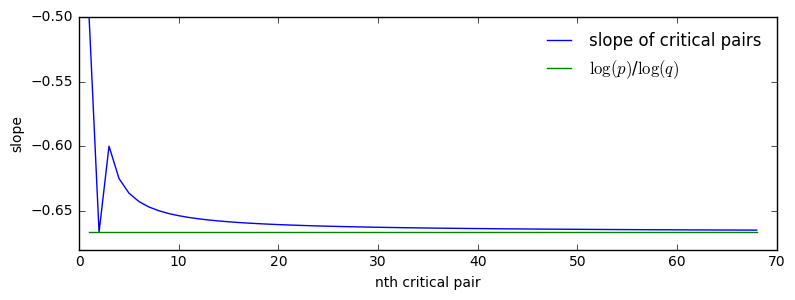
\includegraphics[scale=0.6]{critical_slopes3.png}
%\end{center}
\end{frame}
%%%%%%%%%%%%%%%%%%%%%%%%%%%%%%%%%%%%%%%%%%%%%%%%%%%%
\begin{frame}{Converging Ratios}%Why is the graph negative?

As $k \to \infty$, we see that $\frac{n_k}{m_k} \to -\frac{\log p}{\log q}$. 

\begin{center}
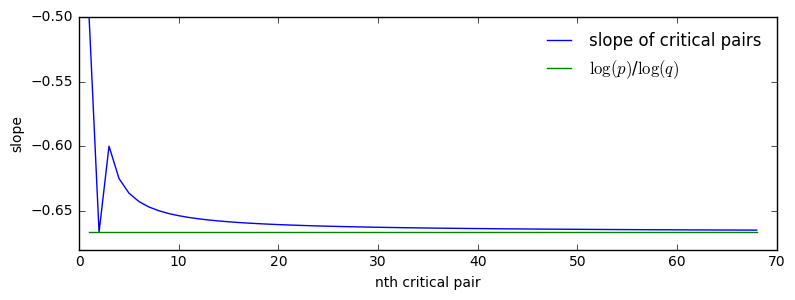
\includegraphics[scale=.75]{critical_slopes3.png}
\end{center}
\end{frame}
%%%%%%%%%%%%%%%%%%%%%%%%%%%%%%%%%%%%%%%%%%%%%%%%%%%%
\section{Results}
\begin{frame}{Two Primes}
After developing an understanding for the problem, we began to analyze the details that Erd\"os glossed over. This lead us to a proof for the following theorem:\\
\begin{block}{Theorem 1}
\textit{For any two distinct prime numbers $p$, and $q$, there exist infinitely many critical pairs.}
\end{block}

\end{frame}
%%%%%%%%%%%%%%%%%%%%%%%%%%%%%%%%%%%%%%%%%%%%%%%%%%%%
\begin{frame}{Key Lemmas}
    \begin{block}{Lemma 4}
        \textit{Consider the pure powers $p^a, q^b$ with $p^a < q^b$ and $a,b \in \Z^+$. If, for all critical pairs $p^s,q^t$ with $s<a$ and $t<b$, $$1<\frac{q^b}{p^a}<\frac{q^t}{p^s}, \quad s,t \in \Z^+$$ then $p^a, q^b$ is a critical pair.}
    \end{block}
    A sketch of the proof follows.
\end{frame}

Assume that for all critical pairs $p^s,q^t$ with $s<a$ and $t<b$, 
$$1<\frac{q^b}{p^a}<\frac{q^t}{p^s},$$ and suppose for contradiction that $p^a, q^b$ is not a critical pair. Since $p^a, q^b$ is not a critical pair, then there exists an intermediate mixed power of the form
$$p^a < q^{b-\tilde{b}}p^{\tilde{a}} < q^b$$
So, since $p^a < q^{b-\tilde{b}}p^{\tilde{a}}$, 
\[\frac{q^b}{p^a}>\frac{q^b}{q^{b-\tilde{b}}p^{\tilde{a}}}=\frac{q^\tilde{b}}{p^\tilde{a}}.\]
If $p^{\tilde{a}}$ and $q^{\tilde{b}}$ are a critical pair, we have a contradiction. If not, repeat.

%%%%%%%%%%%%%%%%%%%%%%%%%%%%%%%%%%%%%%%%%%%%%%%%%%%%
\begin{frame}{Key Lemmas} 
    \begin{block}{Dirichlet's Approximation Theorem}
    Let $\alpha$ be a real number. Given any $\epsilon>0$, there exist M, N $\in \Z$ such that
    $$ \left| \alpha - \frac{M}{N}\right|<\epsilon.$$
    \end{block}
\end{frame}

%%%%%%%%%%%%%%%%%%%%%%%%%%%%%%%%%%%%%%%%%%%%%%%%%%%%
\begin{frame}{The "Tail" of the Sequence of Exponents}%Another frame
\begin{center}

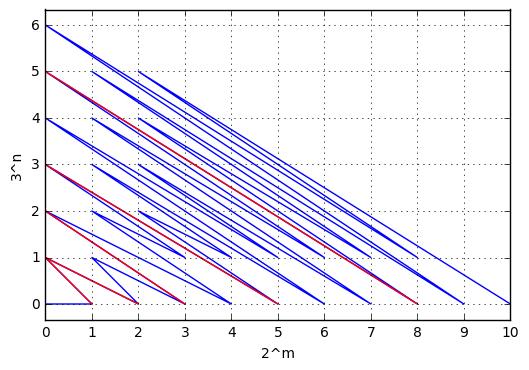
\includegraphics[scale=.48]{slope_plot4.png} 

By the way, the fact that as $k \to \infty$, $\frac{n_k}{m_k} \to -\frac{\log p}{\log q}$. \\ follows from Dirichlet's Approximation Theorem and Lemma 4. 
\end{center}

%\begin{center}
%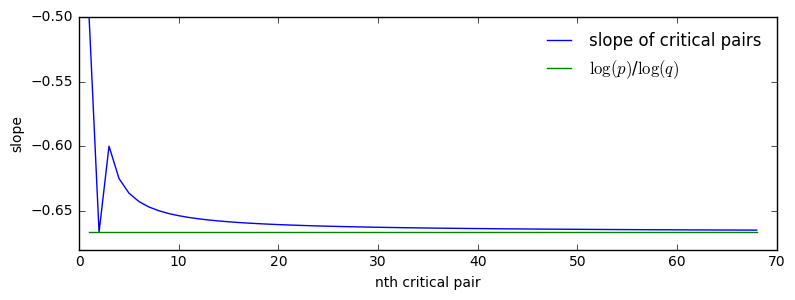
\includegraphics[scale=0.6]{critical_slopes3.png}
%\end{center}
\end{frame}

%%%%%%%%%%%%%%%%%%%%%%%%%%%%%%%%%%%%%%%%%%%%%%%%%%%%
\begin{frame}{Key Lemmas} 
    \begin{block}{Dirichlet's Approximation Theorem}
    Let $\alpha$ be a real number. Given any $\epsilon>0$, there exist M, N $\in \Z$ such that
    $$ \left| \alpha - \frac{M}{N}\right|<\epsilon.$$
    \end{block}
    
    \begin{block}{Lemma 5}
        Let $\alpha$ be an irrational number. Given any $\epsilon > 0$, there exists an $n \in \N$ such that $n\alpha-\floor{n\alpha}<\epsilon$.
    \end{block}
\end{frame}

%%%%%%%%%%%%%%%%%%%%%%%%%%%%%%%%%%%%%%%%%%%%%%%%%%%%    
\begin{frame}{Proof of the Result}
    Let $p$ and $q$ be distinct primes. Suppose for contradiction that there exist finitely many critical pairs. Of these critical pairs, consider the critical pair with $p^{k} < q^{\ell}$ such that $\frac{q^{\ell}}{p^{k}}$ is smallest. This means that 
$$1 < \frac{q^{\ell}}{p^{k}}.$$
Choose some $\epsilon\in\R$ such that 
$$1<p^\epsilon<\frac{q^{\ell}}{p^{k}}.$$
Now, consider the irrational number $\log_pq$. By Lemma 5, there exists some $\Omega\in\N$ such that 
$$\Omega\log_pq - \floor{\Omega\log_pq} < \epsilon.$$
\end{frame}

%%%%%%%%%%%%%%%%%%%%%%%%%%%%%%%%%%%%%%%%%%%%%%%%%%%%    
\begin{frame}{Proof of the Result}


To simplify the notation, let $a=\floor{\Omega\log_pq}$. Thus, with a little algebra, 
\[\arraycolsep=1.4pt\def\arraystretch{1.5}
\begin{array}{rclcl}
\Omega\log_pq - a &<& \epsilon\\
\Omega\log_pq 	&<&a+\epsilon\\
q^\Omega 		&<& p^{a}p^\epsilon\\
\dfrac{q^\Omega}{p^a}&<&\hspace{7pt}p^\epsilon&<&\frac{q^{\ell}}{p^{k}}\\
%\dfrac{q^\Omega}{p^a} &<&\frac{q^{\ell}}{p^{k}}\\
\end{array}
\]
%$$\dfrac{q^\Omega}{p^a}<p^\epsilon<\frac{q^{\ell}}{p^{k}}$$
Hence,
$$1<\dfrac{q^\Omega}{p^a}<\frac{q^{\ell}}{p^{k}}.$$
Therefore, by Lemma 4, $({q^\Omega},{p^a})$ is a critical pair with ratio closer to 1, which is a contradiction. 
    
\end{frame}
%%%%%%%%%%%%%%%%%%%%%%%%%%%%%%%%%%%%%%%%%%%%%%%%%%%%
\begin{frame}{Redeveloped Proof}
       
    \begin{block}{Problem}
    Everything depends on
    $$1<\dfrac{q^\Omega}{p^a}<\frac{q^{\ell}}{p^{k}}.$$
    \end{block}

\end{frame}
%%%%%%%%%%%%%%%%%%%%%%%%%%%%%%%%%%%%%%%%%%%%%%%%%%%%
%%%%%%%%%%%%%%%%%%%%%%%%%%%%%%%%%%%%%%%%%%%%%%%%%%%%
%\begin{frame}{Geometric Intuition}
%    \begin{columns}
%    \begin{column}{.5\textwidth}
%    It is a consequence of Dirichlet's Lemma that there exist infinitely many integers $M,N$ such that 
%    $$\left| \frac{M}{N}-\frac{\log p}{\log q}\right|=\frac{1}{2N^2} _.$$
%    
%    Notice that there are no integer $y$ values in $y = M - \frac{M}{N}k$
%    \end{column}
%    \begin{column}{.5\textwidth}
%    \includegraphics[width=\textwidth]{every_open_%cover_has_a_finite_subcover}
%    \end{column}
%    \end{columns}
%\end{frame}
%%%%%%%%%%%%%%%%%%%%%%%%%%%%%%%%%%%%%%%%%%%%%%%%%%%%
\section{What Next?}
\begin{frame}{Issues with 3 Primes}

    We have attempted the problem with various techniques: Mean Value Theorem/Taylor Polynomial bounds, Geometric Arguments, Linear Programming, Special cases (59,61,3601, (p,q,r = pq +2)), etc.
    
\end{frame}
%%%%%%%%%%%%%%%%%%%%%%%%%%%%%%%%%%%%%%%%%%%%%%%%%%%%
\begin{frame}{Moving Forward}
Currently, we are continuing to look into our geometric argument in three dimensions. 
\end{frame}
%%%%%%%%%%%%%%%%%%%%%%%%%%%%%%%%%%%%%%%%%%%%%%%%%%%%
\begin{frame}{Acknowledgments}
    Thank you to our advisor Dr. Werner Horn for overseeing this project, as well as Dr. Helena Noronha and the rest of the PUMP program for providing us with this opportunity. \vspace{.1in}
        
    Thank you to the NSF for providing funding through the  PUMP program award, NSF Grant DMS-1247679.
    
    \begin{center}
        \includegraphics[scale = .3]{NSFLogo.png}
        \includegraphics[scale = .5]{CSUNlogo.png}
    \end{center}
\end{frame}
%%%%%%%%%%%%%%%%%%%%%%%%%%%%%%%%%%%%%%%%%%%%%%%%%%%%
\end{document}